\documentclass[a4paper, 12pt, notitlepage]{article}
\usepackage[margin=0.5in]{geometry}
\usepackage[english]{babel}
\usepackage[utf8x]{inputenc}
\usepackage{fancyhdr}
\usepackage{amsmath}
\usepackage{amssymb}
\usepackage{gensymb}
\usepackage[makeroom]{cancel}
\usepackage{newfloat}
\usepackage{pdfpages}
\usepackage{graphicx}
\usepackage{tabularx}
\usepackage{array}
\usepackage{hyperref}

\title{Computational Biology - 1$^\text{st}$ Assignment}
\author{Nicolás Espinoza Muñoz}
\date{October 3, 2020}

\newcommand\numberthis{\addtocounter{equation}{1}\tag{\theequation}}
\pagenumbering{gobble}

\begin{document}
\maketitle
\subsection*{Introduction}
This work involves numerical trials made in order to better understand the means by which scientists obtain solutions - more correctly, solution approximations - of quantum systems. We will use harmonic oscillator basis functions to approximate different Hamiltonian operators ($\hat{H}$). The first question (number 3 in the problems presentation) is the only one solved both analytically and numerically. Every solution is presented in the annexed \texttt{Mathematica} notebook, and we merely show and quickly explain said results in this text. This work will be developed using the  basis functions of a harmonic oscillator (Eq. (\ref{eq:eq1})) and, most of the time, the harmonic oscillator's Hamiltonian operator in atomic units
\begin{equation*}
	H_0 = \frac{1}{2}(p² + q²)
\end{equation*}
\subsection*{3.}
First we are asked basically to prove that the inner product of harmonic oscillator basis functions produce an unitary matrix. These functions are defined by
\begin{equation}
	\phi_j(q) = \left(2^jj!\sqrt{\pi}\right)^{-1/2}e^{-q^2/2}\mathcal{H}_j(q)\label{eq:eq1}
\end{equation}
The terms in the \_\_\_\_\_\_\_ matrix are defined by
\begin{equation}
	\langle \phi_i|\phi_j \rangle = \int_{-\infty}^{\infty}\phi_i(q)\phi_j(q)\, dq = \int_{-\infty}^{\infty}\frac{e^{-q^2}\mathcal{H}_i(q)\mathcal{H}_j(q)}{\left(2^jj!\sqrt{\pi}\cdot 2^ii!\sqrt{\pi}\right)^{-1/2}}\, dq \label{eq:eq2}
\end{equation}
The denominator in the fraction is a constant with respect to $q$, so we can ignore it for now. Since $\mathcal{H}_j$ is the Hermite polynomial of order $j$, it suffices to prove that said polynomials are orthogonal. The Hermite polynomials are defined by
\begin{equation*}
	\mathcal{H}_j(q) = (-1)^je^{q^2}\frac{d^j}{dq^j}\left(e^{-q^2}\right)
\end{equation*}
so now we proceed to the calculation of the inner product using the weight function $w(q) = e^{-q^2}$.
\begin{align*} \int_{-\infty}^{\infty}\mathcal{H}_i(q)\mathcal{H}_j(q) e^{-q^2}\,dq & = \int_{-\infty}^{\infty}(-1)^i\cancel{e^{q^2}}\cdot \cancel{e^{-q^2}}\frac{d^i}{dq^i}\left(e^{-q^2}\right)\mathcal{H}_j(q)\,dq\\
&= (-1)^i\int_{-\infty}^{\infty}\mathcal{H}_j(q)\frac{d^i}{dq^i}\left(e^{-q^2}\right)\, dq\numberthis\label{eq:eq3}
\end{align*}
Now for $i>j$, we integrate by parts. Ignoring the $(-1)^i$ term for now in Eq. (\ref{eq:eq3}), we get
\begin{equation}
	\int_{-\infty}^\infty\mathcal{H}_j(q)\frac{d^i}{dq^i}\left(e^{-q^2}\right)\, dq = \left.\mathcal{H}_j(q)e^{-q^2}\right|_{-\infty}^{\infty} - \int_{-\infty}^{\infty}e^{-q^2}\frac{d^i}{dq^i}\mathcal{H}_j(q)\, dq\label{eq:eq4}
\end{equation}
The first term of the right hand side is always zero due to the exponential. The integral term of the RHS is zero for the condition specified $i>j$. Thus, only the terms corresponding to the lower triangular portion of the matrix remain. By switching the $i$ and $j$ indexes, it can be shown that also the upper triangular portion of the matrix is zero. The only non-zero elements in the matrix are those in the diagonal. For $i=j$, Eq. (\ref{eq:eq3}) results in
\begin{equation*}
	j!2^j\sqrt{\pi}
\end{equation*}
The denominator in Eq. (\ref{eq:eq2}) for $i = j$ becomes simply $2^jj!\sqrt{\pi}$. Replacing our latest result in said equation shows that every term in the diagonal of the $\langle\phi_j|\phi_i\rangle$ matrix is $1$, therefore proving that it corresponds to the unitary matrix.\\\\
\subsubsection*{Matrix result}
We were asked to show the matrix form of the previous result, proving by doing so that the first integral of Eq. (\ref{eq:eq2}) gives the identity or unitary matrix. The result is given in the annexed notebook (Espinoza\_Nicolas.nb). The form is an $i\times j$ matrix like this
\begin{equation*}
	\begin{bmatrix}
		1 & 0 & 0 & \dots & 0 \\
		0 & 1 & 0 & \dots & 0 \\
		0 & 0 & 1 & \dots & 0 \\
		\vdots & \vdots & \vdots & \ddots & \vdots \\
		0 & 0 & 0 & \dots & 1
	\end{bmatrix}
\end{equation*}
\subsection*{4.}
When applied over the basis function $\varphi_j$, and then multiplied by the conjugate $varphi_i$ and integrated over all space, the Hamiltonian operator $H_0$ can be expressed in a matrix form that allows for calculation of the Eigenvalues of the system, which in turn correspond to the energy levels of the analyzed particle. It is proven in the annexed notebook that the inner function product of $\varphi_i\cdot H_0(\varphi_j) \neq 0$ only for $i=j$, and therefore is a diagonal matrix without need for matrix operations attempting diagonalization.\\\\
The resulting matrix, computed for the 10 first energy levels, is coherent to what is stated in the problems presentation, where it is explained that all diagonal elements follow a recurrence relation of the form
\begin{equation*}
	\varepsilon_j⁰ = j + \frac{1}{2}\qquad j =0,1,2...
\end{equation*}
A portion of the matrix is shown below, for reference
\begin{equation*}
\begin{bmatrix}
1/2 & 0 & 0 & \dots & 0 \\
0 & 3/2 & 0 & \dots & 0 \\
0 & 0 & 5/2 & \dots & 0 \\
\vdots & \vdots & \vdots & \ddots & \vdots \\
0 & 0 & 0 & \dots & 19/2
\end{bmatrix}
\end{equation*}
\subsection*{5.}
We are now asked to proceed with the calculation of two operators in matrix form with the basis functions of an harmonic oscillator. These new operators, for any function $f$, are the \textit{relative position} ($q = q\cdot(f)$) and \textit{linear momentum} ($p = -i\cdot \frac{d}{dq}(f)$). The results are as follows (also in the notebook):\\\\
For the $q$ operator:
\begin{equation*}
\begin{bmatrix}
	0 & 1/\sqrt{2} & 0 & 0 & 0 & 0 & 0 & 0 &  \\
	1/\sqrt{2} & 0 & 1 & 0 & 0 & 0 & 0 & 0 & \\
	0 & 1 & 0 & \sqrt{3/2} & 0 & 0 & 0 & 0 & & \\
	0 & 0 & \sqrt{3/2} & 0 & \sqrt{2} & 0 & 0 & 0 & \dots \\
	0 & 0 & 0 & \sqrt{2} & 0 & \sqrt{5/2} & 0 & 0 & \\
	0 & 0 & 0 & 0 & \sqrt{5/2} & 0 & \sqrt{3} & 0 & \\
	0 & 0 & 0 & 0 & 0 & \sqrt{3} & 0 & \sqrt{7/2} &  \\
	& & & & \vdots
\end{bmatrix}
\end{equation*}
And for the $p$ operator:
\begin{equation*}
\begin{bmatrix}
	0 & -i/\sqrt{2} & 0 & 0 & 0 & 0 & 0 & 0 &  \\
	i/\sqrt{2} & 0 & -i & 0 & 0 & 0 & 0 & 0 & \\
	0 & i & 0 & -\sqrt{3/2}\,i & 0 & 0 & 0 & 0 & & \\
	0 & 0 & \sqrt{3/2}\,i & 0 & -\sqrt{2}\,i & 0 & 0 & 0 & \dots \\
	0 & 0 & 0 & \sqrt{2}\,i & 0 & -\sqrt{5/2}\,i & 0 & 0 & \\
	0 & 0 & 0 & 0 & \sqrt{5/2}\,i & 0 & -\sqrt{3}\,i & 0 & \\
	0 & 0 & 0 & 0 & 0 & \sqrt{3}\,i & 0 & -\sqrt{7/2}\,i &  \\
	& & & & \vdots
\end{bmatrix}
\end{equation*}
\subsection*{6.}
We can replicate the Hamiltonian operator presented in the introduction to this work by expressing both operators $q$ and $p$ separately in matrix form, and then taking the matrix product and adding them
\begin{equation}
	\underline{H_0} = \frac{1}{2}(\underline{p²} + \underline{q²}) \approx \frac{1}{2}(\underline{p}\cdot\underline{p} + \underline{q}\cdot\underline{q})
\end{equation}
where the underline is used to represent a matrix. The result of doing this is an error in the last diagonal element of the matrix, which greatly deviates from the analytical value due to the truncation of the expansion approximating the Hamiltonian of the harmonic oscillator. We show in the notebook that this error becomes larger for the last term, as the number of basis functions grows. As a remark, this was only tried for three matrix sizes chosen arbitrarily, and was left without running on the notebook for presentation purposes.

\subsection*{7.}
\subsubsection*{a)}
-
\subsubsection*{b)}
We chose 10 amounts of basis functions for this, from 10 to 28 (both included) in steps of 2. The energies were calculated and plotted in the next 4 panels. From left to right, the upper panels have the three highest energies for all basis functions ($\varepsilon_6$, $\varepsilon_5$, $\varepsilon_4$ and $\varepsilon_3$) and the next one has $\varepsilon_2$. The two lower panels have $\varepsilon_1$ and $\varepsilon_0$. This way of visualizing was chosen due to the big differences in energy scales.\\
\begin{figure}[!h]
	\centering
	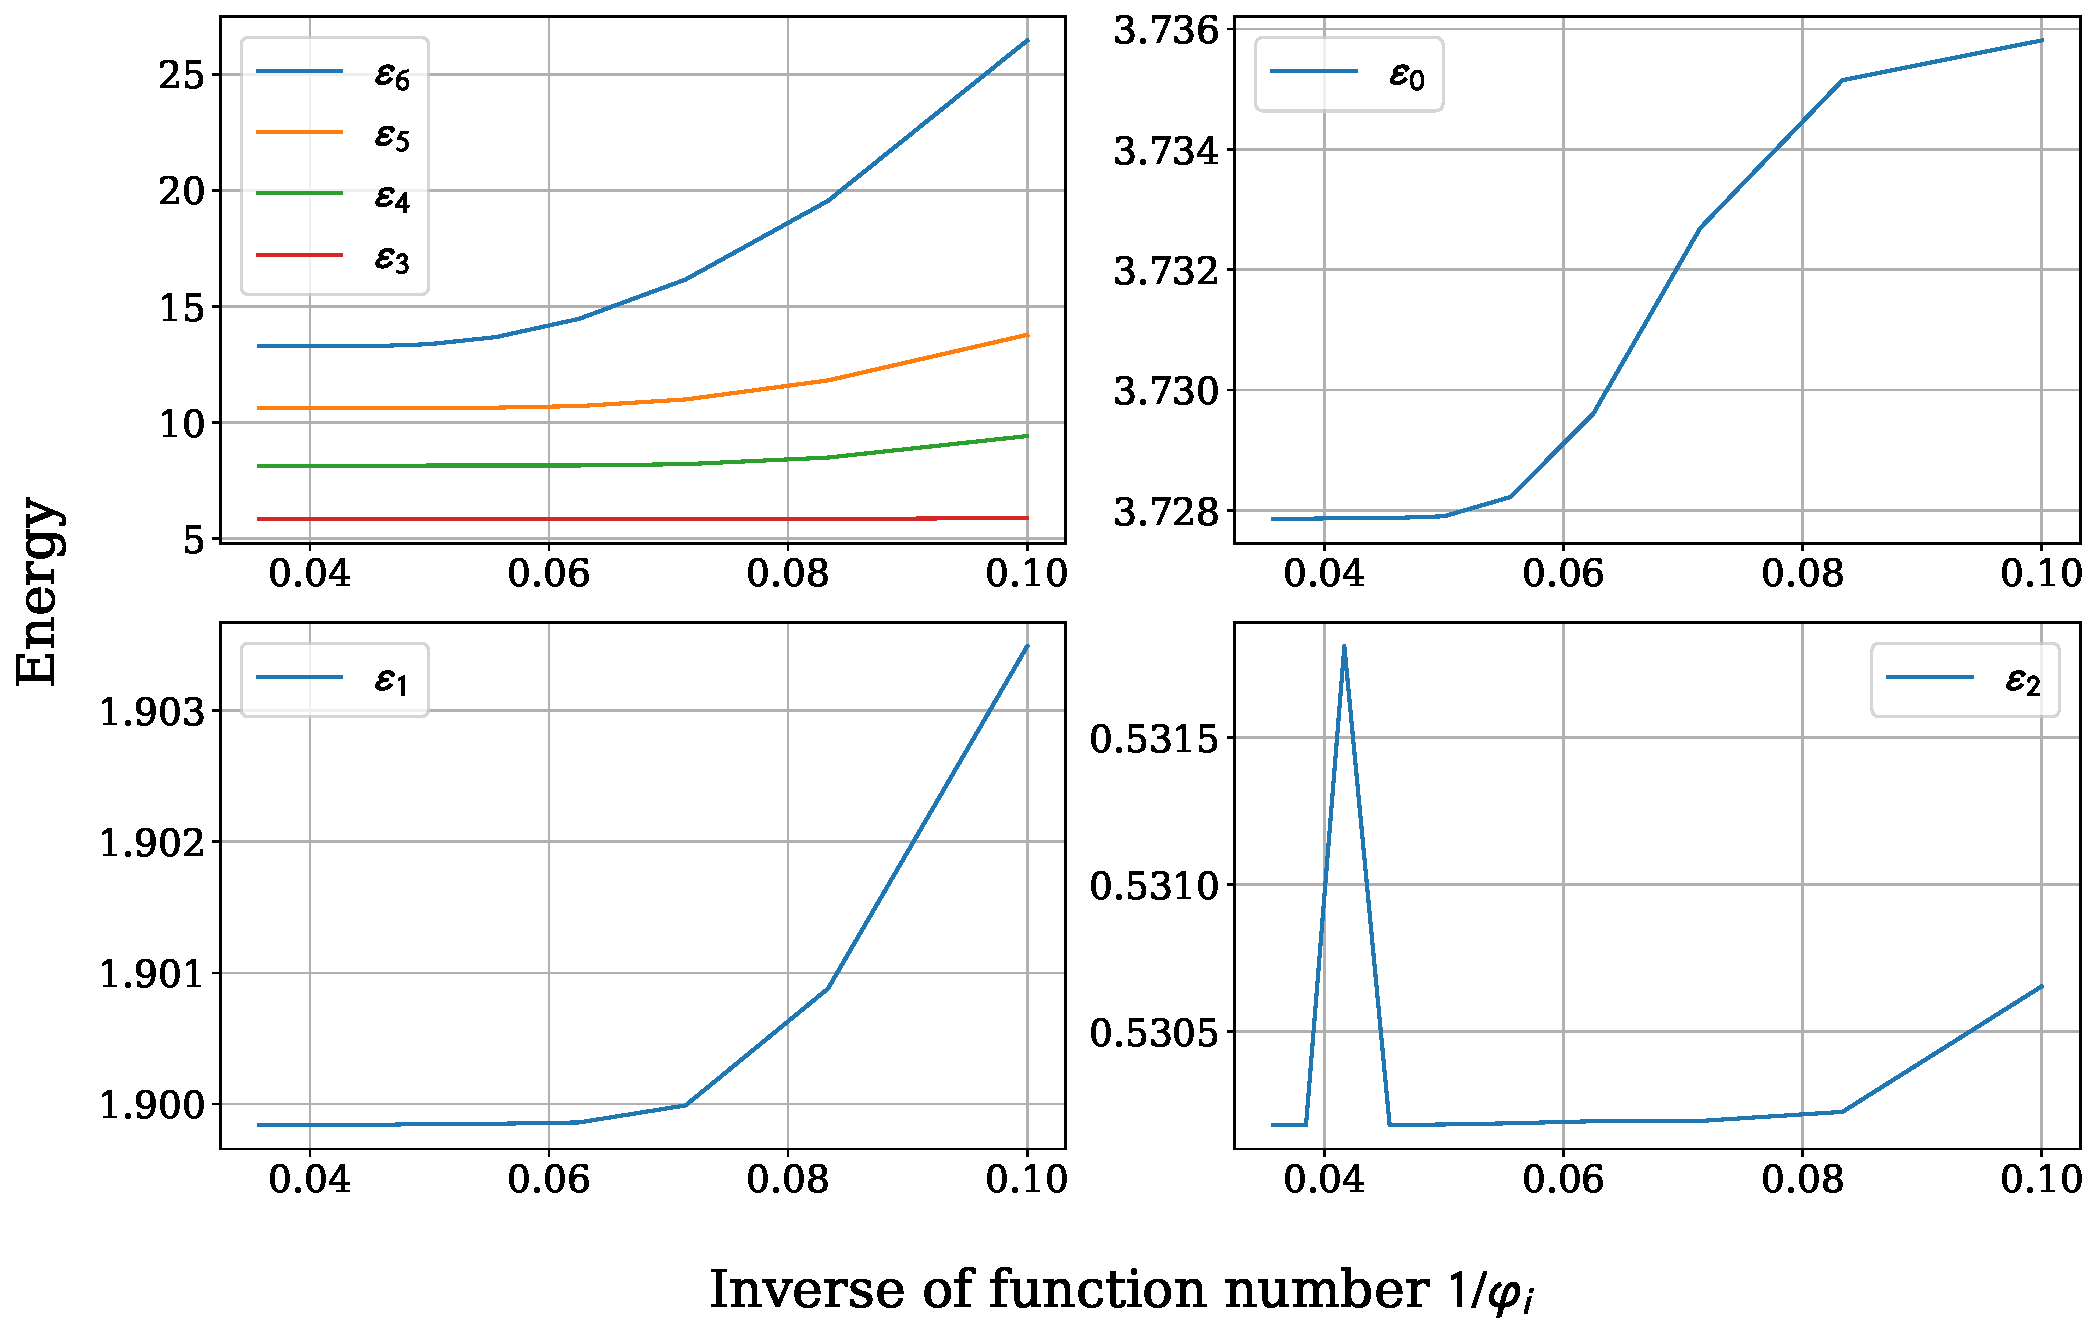
\includegraphics[scale=0.5]{Figures/plot2.pdf}
	\caption{Plots of energy as a function of number of basis functions used to calculate said energy.}
\end{figure}
\subsubsection*{c)}
We were asked to find out how many basis functions are needed to reach an error value of $0.01\%$ when compared to exact values. We stopped at 35 basis functions, because there was no real improvement in the convergence by that point, at least based on what we could detect; that is to say, values between iterations weren't changing noticeably. The error with 35 basis functions is shown in the next table (both the value and the calculated relative error)
\begin{table}
	\begin{tabular}[ccccccccc]
	& $\varepsilon_0$ & $\varepsilon_1$ & $\varepsilon_2$ & $\varepsilon_3$ & $\varepsilon_4$ & $\varepsilon_5$ & $\varepsilon_6$
%	Value & 
%	Error & 
	\end{tabular}
\end{table}
\end{document}